\documentclass{article}

\usepackage{fouche}
\author{}
\date{}
\title{Problema (da presentare in forma aperta)}
\begin{document}
\maketitle
\noindent
Fosco Loregian \hfill A-26
\subsection{Esecuzione del disegno}
Costruire un segmento AB 
\begin{itemize}
  \item Si scelgono due punti nel piano (usando due volte lo strumento {\tt Punto})
  \item si traccia la retta tra loro (usando lo strumento {\tt Retta per due punti})
\end{itemize}
e un punto C in modo che C non appartenga alla retta di AB.
\begin{itemize}
  \item Si sceglie lo strumento {\tt Punto}
  \item si costruisce la parallela ad $AB$ passante per $C$ con lo strumento {\tt retta parallela a un punto dato}
\end{itemize}
Costruire un quadrilatero ABCD 
\begin{itemize}
  \item \dots con lo strumento {\tt Poligono}
  \item si ottiene la figura seguente:
  \begin{center}
    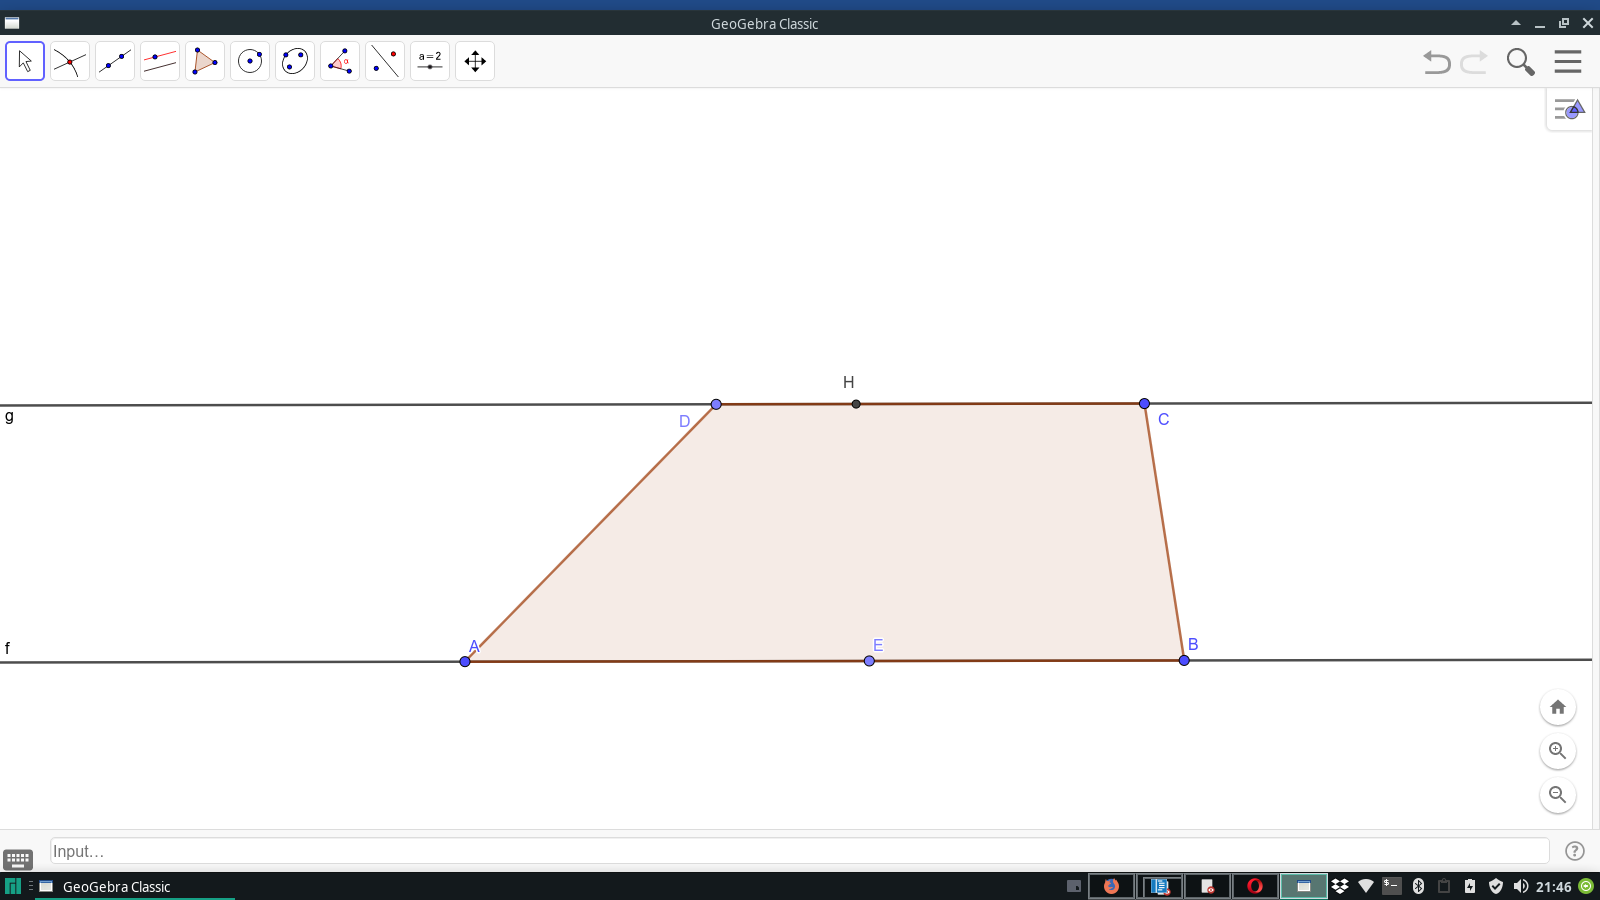
\includegraphics[width=.75\textwidth]{quadril.png}
  \end{center}
\end{itemize}
Ora $D$ è un punto scelto sulla retta parallela a $BC$ passante per $A$.
\subsection{Esame della costruzione}
\begin{itemize}
  \item Ovviamente, il quadrilatero $ABCD$ resterà sempre un trapezio;
  \item si può provare a ragionare su quali condizioni gli fanno mantenere la stessa area (o lo stesso perimetro, ma queste sono più tediose);
  \item si può provare a ragionare sulle condizioni di parallelismo tra $AC$ e $BD$;
  \item si può provare a riscoprire il teorema di Pappo-Pascal: si sceglie un punto $E$ su $AB$, si tracciano le rette $ED$ ed $EC$: ora, per ogni $H$ su $CD$, i punti di intersezione $AD\land BC$, $AH\land EC$ e $BH\land ED$ nella costruzione che segue sono allineati:
\begin{center}
  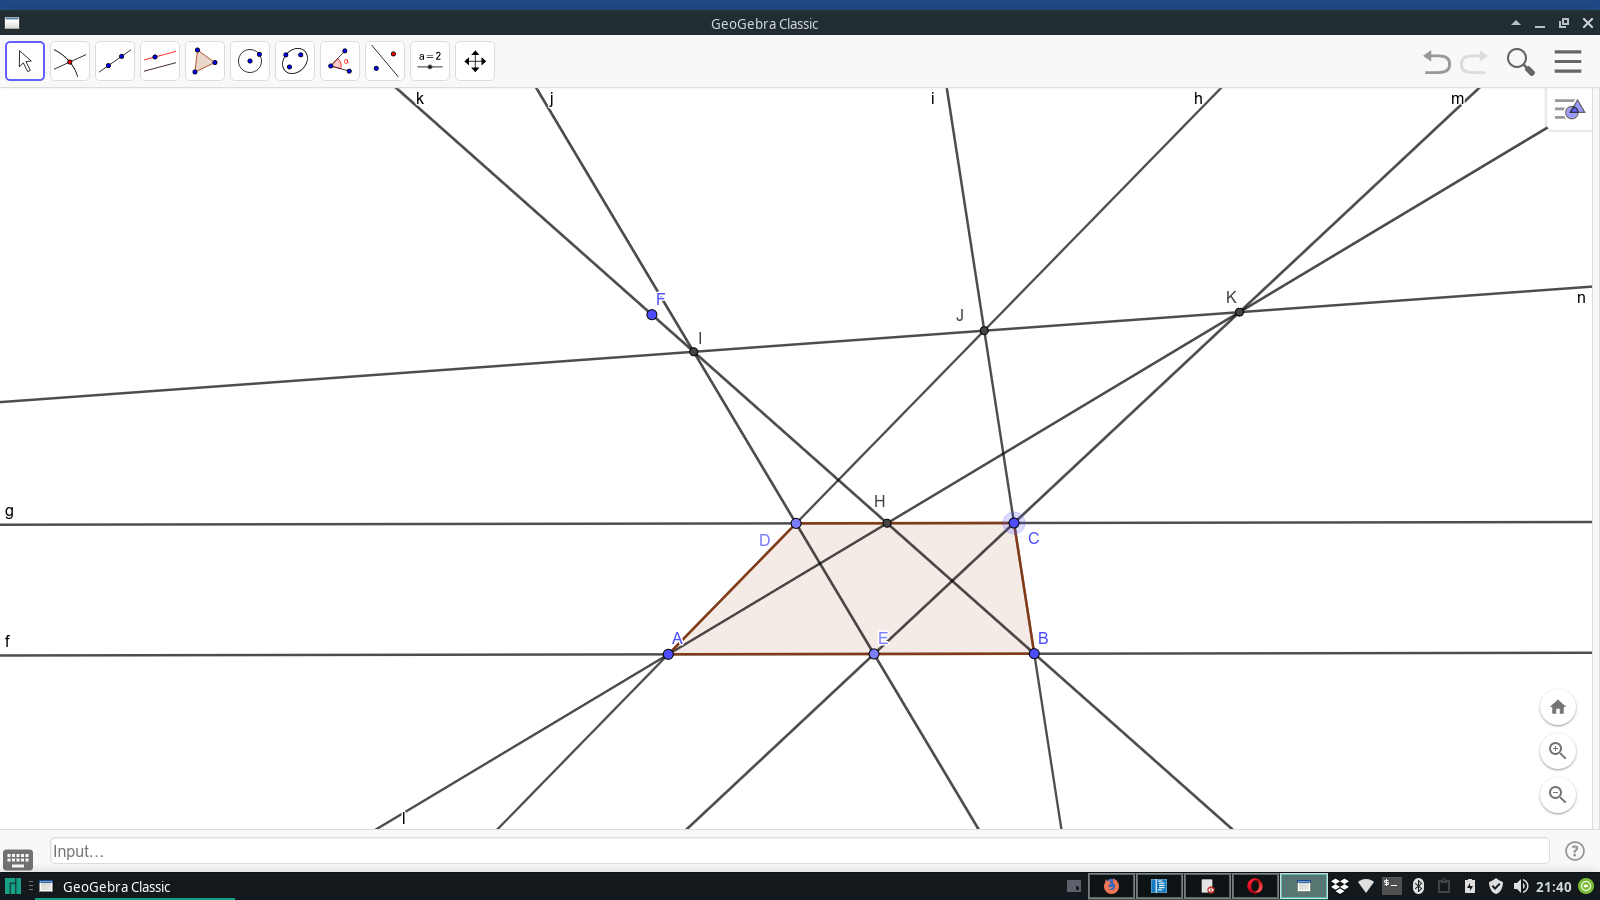
\includegraphics[width=.75\textwidth]{pap.png}
\end{center}
Si può provare a spostare il punto $E$ e vedere come la costruzione muta di forma, ma la relazione di allineamento permane. Si può provare ad argomentare perché i punti $J,H,E$ non siano collineari.
\end{itemize}
\end{document}